\documentclass[]{article}

\usepackage{listings}
\usepackage{graphicx}
\usepackage{subcaption}

% Title Page
\title{CSC2541 - Problem Set 1}
\author{Sumeet Ranka}

\lstset{breaklines=true, basicstyle=\ttfamily}

\begin{document}
\maketitle

\section*{Part 1}
1. With respect to the columns in the table \texttt{admissions}, the patient with id = $40080$ is a African-American widowed woman. She lived for 79 years. Her religious beliefs are unknown. She can speak Hait. 

\begin{lstlisting}[]
select * from admissions,patients where admissions.subject_id=`40080' and patients.subject_id=`40080';
\end{lstlisting}

2. The patient was primarily diagnosed for the condition: \textit{Acute on chronic combined systolic and diastolic heart failure}. The corresponding ICD9 Code is 42843.

\begin{lstlisting}[]
select * from d_icd_diagnoses where icd9_code=(select icd9_code from diagnoses_icd where subject_id=`40080' and seq_num=1);
\end{lstlisting}

3. She was admitted in the ICU for approximately 5 days (to be exact 4.8577 days). She was discharged with a minimally clear and coherent mental status. She had a minimally alert and somewhat interactive level of consciousness. She was reported to be bed bound and a dependent hemiplegia.

\begin{lstlisting}[]
select * from noteevents where subject_id=`40080' order by chartdate desc,charttime desc;
\end{lstlisting}
 
4. The highest heart rate recorded is 141 and the lowest heart rate is 80. 

\begin{lstlisting}[]
select min(valuenum), max(valuenum) from chartevents where itemid in (select itemid from d_items where label=`Heart Rate') and subject_id=`40080';
\end{lstlisting}

\section*{Part 2}
\textbf{2a.} The following columns are dropped after splitting the data into training and validation set:

\begin{itemize}
	\item train
	\item subject\_id
	\item hadm\_id
	\item icustay\_id
	\item mort\_icu
\end{itemize}

The numerical-valued columns are min-max normalized before feeding into the logistic regression model. 

After the above stated preprocessing, the AUC Score obtained is $0.7709$. Figure \ref{fig:roc2a} shows the ROC Graph obtained.

\begin{figure}
	\centering
	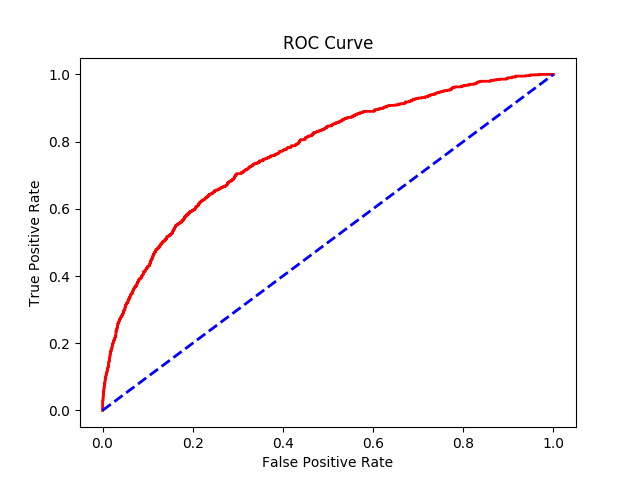
\includegraphics[width=0.8\linewidth]{ROC_part2a.png}
	\caption{ROC Graph for model trained on \texttt{adult\_icu.gz} for predicting mortality}
	\label{fig:roc2a}
\end{figure}

To compare the coefficients, the absolute values of the corresponsing weights are considered. The top 5 and lowest 5 risk factors obtained are mentioned in the table \ref{tab:2a}.

\begin{table}[t]
	\centering
	\begin{tabular}{|c|c|}
		\hline
		\textbf{Top 5} & \textbf{Lowest 5}\\
		\hline
		bilirubin (+) & admType\_NEWBORN\\
		lactate (+) & glucose\_mean\\
		tempc\_min (-) & eth\_asian\\
		tempc\_max (+) & ptt\\
		creatinine (-) & eth\_white\\
		\hline
	\end{tabular}
	\caption{Top 5 and Lowest 5 risk factors associated with mortality. The sign indicates whether the factor is positively or negatively correlated.}
	\label{tab:2a}
\end{table}

The model takes 11 iterations to converge when the data is standardized. However, it takes 203 iterations if not. The AUC score in the non-standardized case is slightly higher ($0.7768$). However, in this case we cannot comment on the risk factors as the values for every column is not in the same range. From the ROC Curve, we can conclude that the model performes moderately good. It is more accurate than the baseline but not sufficiently steep in the left to make it a deployable model.

The following are the explanation of the top 5 and the lowest 5 mortality factors.
\begin{itemize}
	\item High levels of \texttt{bilirubin} indicates liver inefficiency or indication of diseases such as jaundice.
	\item A general increase in the \texttt{lactate} means a greater severity of the condition. It indicates the concentration of lactate in the blood.
	\item \texttt{tempc\_min} indicates the minimum temperature (in celsius) that the patient had. Lower body temperature means the person may be suffering from hypothermia.
	\item \texttt{tempc\_max} indicates the maximum temperature (in celsius) that the patient had. Higher temperature means the harder your body is working to fight the infection.
%	\item BUN (or Blood Urea Nitrogen) indicates how well the kidneys are working. It is the amount of nitrogen in your blood that comes from the waste product urea. Heart failure, dehydration, or a diet high in protein can also make your BUN level higher.
%	\item \texttt{resprate\_mean} is the mean of the respiratory rate values measured for the patient. A single value indicates the number of breaths the patient takes in a single minute.
	\item \texttt{creatinine} is a waste product from the normal breakdown of muscle tissue. High levels indicate the inefficiency of kidney functioning. 
%	\item \texttt{sysbp\_min} indicates the minimum value in the various readings of the systolic blood pressure.
%	\item Platelet indicates the platelet count. Usually higher the platelet count, better is the health. However, very high is unusual and happens rarely.
%	\item \texttt{tempc\_mean} is the mean of the body temperature readings (in celsius).
	\item \texttt{admType\_NEWBORN}: Boolean variable indicating whether the person admitted is a new born.
	\item \texttt{glucose\_mean}: Mean value of the glucose across all the readings. The glucose level could be controlled for the patients.
	\item \texttt{eth\_asian}: Boolean variable stating whether the patient belongs to asian ethnicity.
	\item \texttt{eth\_white}: Boolean variable stating whether the patient belongs to white ethnicity.
	\item \texttt{ptt}: Partial Thromboplastin Time. It indicates the ability of the body to form blood clots. Some literature points to the fact that high values of ptt increases the mortality rate. However, the patients may be under the medication that controls the clotting ability.
\end{itemize}


\textbf{2b.} \texttt{RegexpTokenizer} is used to tokenize the clinical notes. On training a L1-Regularized Logistic regression model using TF-IDF feature vectors, AUC score of $0.8250$ is observed. The model converged in 16 iterations. Figure \ref{fig:roc2b} shows the ROC Graph obtained. 

\begin{figure}
	\centering
	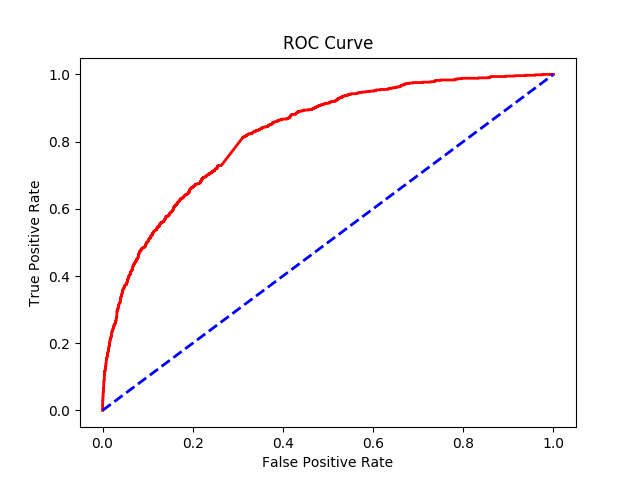
\includegraphics[width=0.8\linewidth]{ROC_part2b.png}
	\caption{ROC Graph for model trained on \texttt{adult\_notes.gz} for predicting mortality}
	\label{fig:roc2b}
\end{figure}

The top five (both positively and negatively correlated) and lowest five words associated with mortality obtained from the data are mentioned in the table \ref{tab:2b}. The word obtained somewhat reflects the condition of the patient. For example, the words like \textit{worsening} and \textit{dnr} reflects a bad condition of the patient whereas words like \textit{extubation} and \textit{good} reflects normal conditions. Words in the last column seems to not hold importance when trying to interpret the condition of the patient.

\begin{table}[t]
	\centering
	\begin{tabular}{|c|c|c|}
		\hline
		\textbf{Top Five Positive} & \textbf{Top Five Negative} & \textbf{Lowest Five}\\
		\hline
		prognosis & diet & 00\\
		cmo & extubation & 000\\
		dnr & clear & 0000\\
		corneal & extubated & 0000am\\
		worsening & good & 0000d\\
		\hline
	\end{tabular}
	\caption{Top Five positively and negatively correlated words and Lowest Five words associated with mortality}
	\label{tab:2b}
\end{table}

\textbf{2c.} Combining the model increases the AUC Score to $0.8471$. The graph is more closer to the left border and the top border. Figure \ref{fig:roc2c} displays the ROC Graph.

\begin{figure}
	\centering
	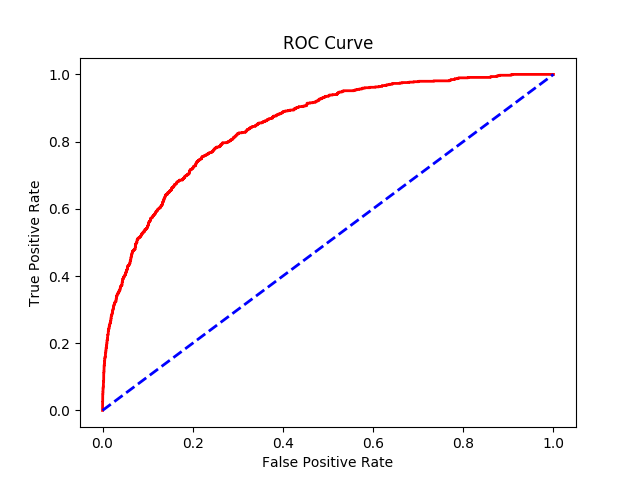
\includegraphics[width=0.8\linewidth]{ROC_part2c.png}
	\caption{ROC Graph for model trained on both \texttt{adult\_icu.gz} and \texttt{adult\_notes.gz} for predicting mortality}
	\label{fig:roc2c}
\end{figure}


\section*{Part 3}

This part deals with the hypertension prediction based on various vital measurements.

\textbf{3a.} AUC Scores and F1 Scores obtained by training a logistic regression model on different feature sets are mentioned in the table \ref{tab:3a}. ROC curves are displayed in the figure \ref{fig:3a}.

\begin{figure*}[t]
	\centering
	\begin{subfigure}[b]{0.475\textwidth}
		\centering
		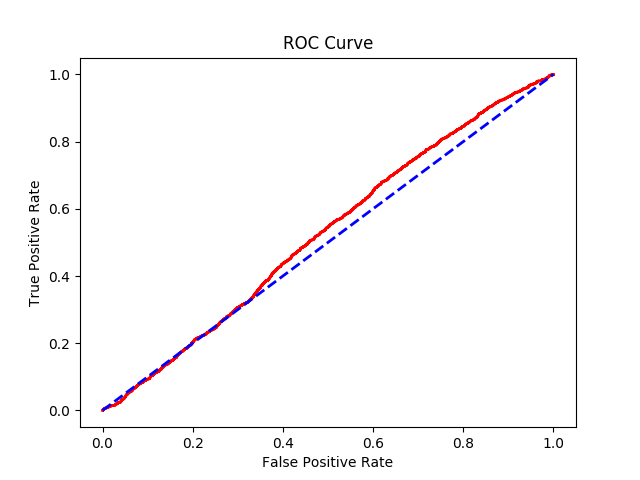
\includegraphics[width=\textwidth]{ROC_part3a_HEART_RATE.png}
		\caption[Heart Rate]%
		{{\small Heart Rate}}    
		\label{fig:3ahr}
	\end{subfigure}
	\hfill
	\begin{subfigure}[b]{0.475\textwidth}  
		\centering 
		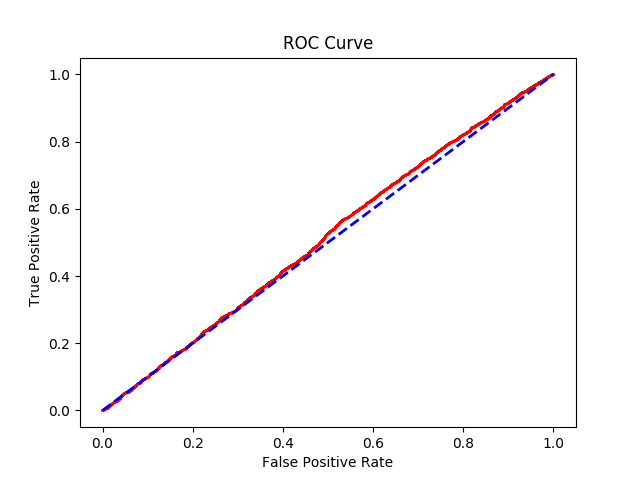
\includegraphics[width=\textwidth]{ROC_part3a_O2_SATURATION.png}
		\caption[]%
		{{\small O2 Saturation}}    
		\label{fig:3ao2}
	\end{subfigure}
	\vskip\baselineskip
	\begin{subfigure}[b]{0.475\textwidth}   
		\centering 
		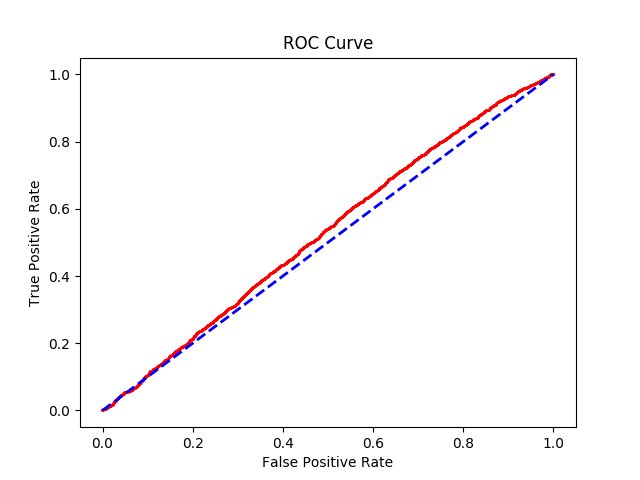
\includegraphics[width=\textwidth]{ROC_part3a_RESPIRATORY_RATE.png}
		\caption[]%
		{{\small Respiratory Rate}}    
		\label{fig:3aresp}
	\end{subfigure}
	\quad
	\begin{subfigure}[b]{0.475\textwidth}   
		\centering 
		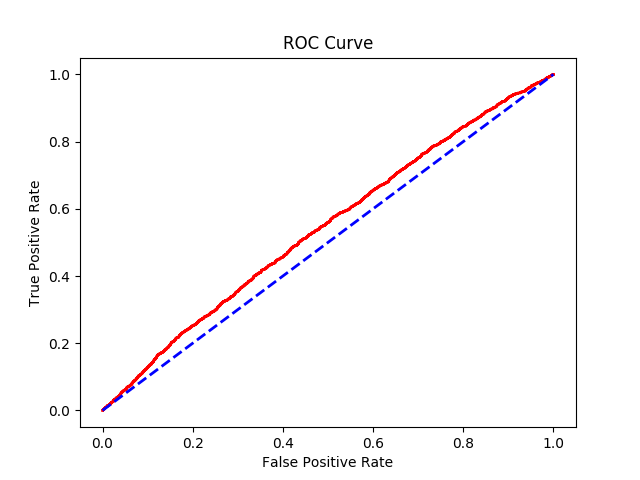
\includegraphics[width=\textwidth]{ROC_part3a_BLOOD_PRESSURE.png}
		\caption[]%
		{{\small Blood Pressure}}    
		\label{fig:3abp}
	\end{subfigure}
	\caption[]
	{\small ROC curves for different feature sets for a trained logistic regression} 
	\label{fig:3a}
\end{figure*}

\begin{table}[h!]
	\centering
	\begin{tabular}{|c|c|c|c|}
		\hline
		\textbf{Feature Set} & \textbf{AUC Score} & \textbf{F1 Score} & \textbf{$\#$ patients removed}\\
		\hline
		Heart Rate & $0.5262$ & $0.0$ & 13\\
		Respiratory Rate & $0.5275$ & $0.0013$ & 16\\
		O2 Saturation & $0.5129$ & $0.0$ & 21\\
		Blood Pressure & $0.5434$ & $0.012$ & 157\\
		\hline
	\end{tabular}
	\caption{AUC Scores and F1 scores obtained by using Logistic Regression to predict hypertension using various feature sets}
	\label{tab:3a}
\end{table}

\textbf{3b.} AUC Scores and F1 Scores obtained by training a LSTM model on different feature sets are mentioned in the table \ref{tab:3b}. ROC Curves are displayed in the figure \ref{fig:3b}.

\begin{table}[h!]
	\centering
	\begin{tabular}{|c|c|c|c|}
		\hline
		\textbf{Feature Set} & \textbf{AUC Score} & \textbf{F1 Score} & \textbf{$\#$ patients removed}\\
		\hline
		Heart Rate & $0.5080$ & $0.0$ & 13\\
		Respiratory Rate & $0.5373$ & $0.0006$ & 16\\
		O2 Saturation & $0.5$ & $0.0006$ & 21\\
		Blood Pressure & $0.51$ & $0.0$ & 157\\
		\hline
	\end{tabular}
	\caption{AUC Scores and F1 scores obtained by using LSTM to predict hypertension using sequences obtained from various feature sets}
	\label{tab:3b}
\end{table}

\begin{figure*}[t]
	\centering
	\begin{subfigure}[b]{0.475\textwidth}
		\centering
		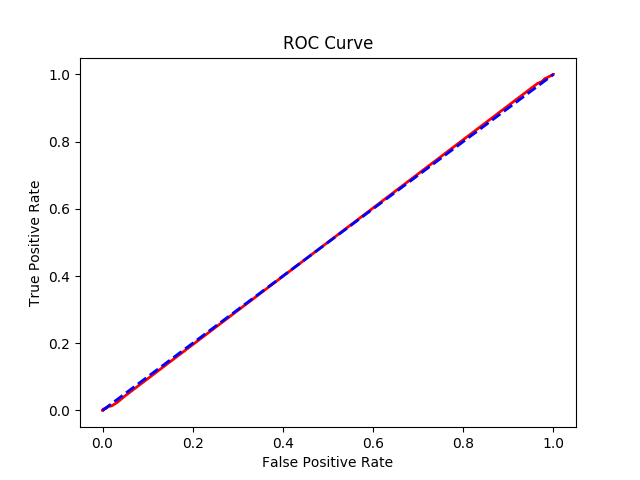
\includegraphics[width=\textwidth]{ROC_part3b_HEART_RATE.png}
		\caption[Heart Rate]%
		{{\small Heart Rate}}    
		\label{fig:3bhr}
	\end{subfigure}
	\hfill
	\begin{subfigure}[b]{0.475\textwidth}  
		\centering 
		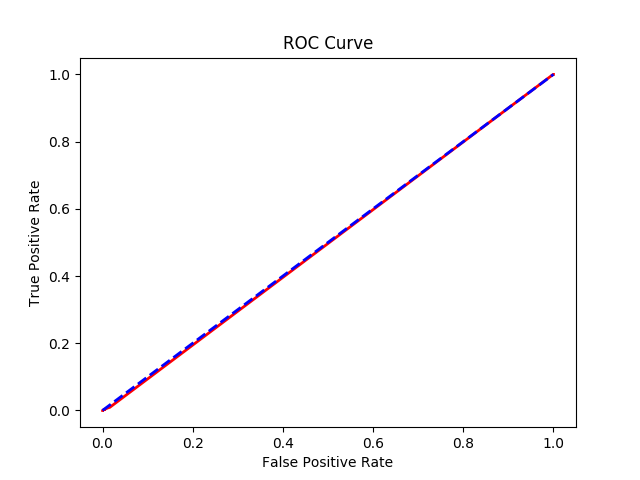
\includegraphics[width=\textwidth]{ROC_part3b_O2_SATURATION.png}
		\caption[]%
		{{\small O2 Saturation}}    
		\label{fig:3bo2}
	\end{subfigure}
	\vskip\baselineskip
	\begin{subfigure}[b]{0.475\textwidth}   
		\centering 
		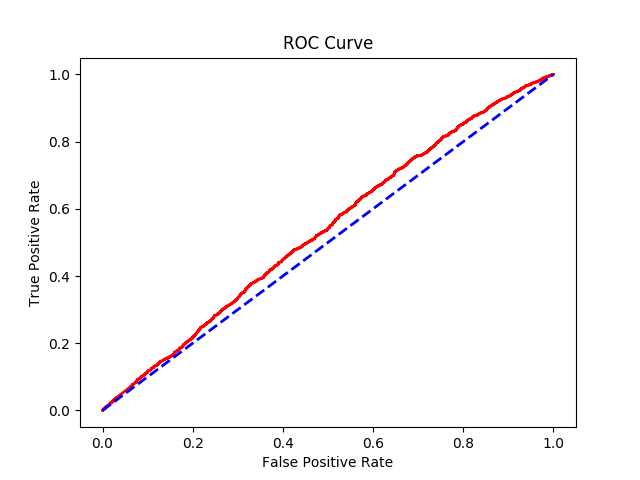
\includegraphics[width=\textwidth]{ROC_part3b_RESPIRATORY_RATE.png}
		\caption[]%
		{{\small Respiratory Rate}}    
		\label{fig:3bresp}
	\end{subfigure}
	\quad
	\begin{subfigure}[b]{0.475\textwidth}   
		\centering 
		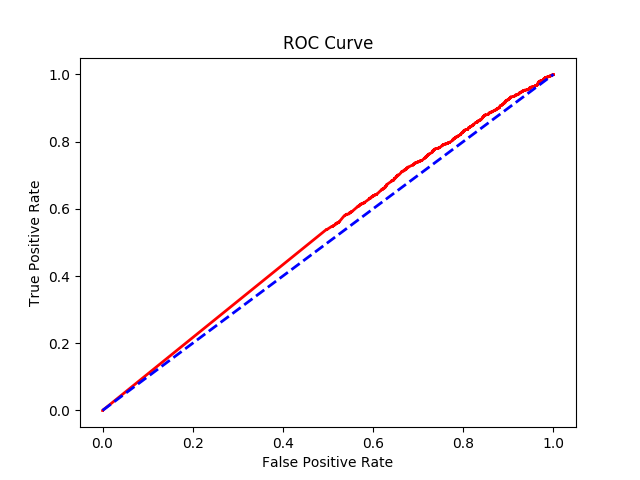
\includegraphics[width=\textwidth]{ROC_part3b_BLOOD_PRESSURE.png}
		\caption[]%
		{{\small Blood Pressure}}    
		\label{fig:3bbp}
	\end{subfigure}
	\caption[]
	{\small ROC curves for different feature sets for a trained LSTM} 
	\label{fig:3b}
\end{figure*}


\textbf{3c.} Based on the performance, none of the models should be used. 

The aggregated values such as min, max and mean do not provide complete information to predict hypertension. 

The sequences provided to LSTM may be overwhelmed by the normal values.

\section*{Part 4}
The text is tokenized using the \texttt{RegexpTokenizer} with the regex \texttt{[a-zA-Z0-9]+}. All the stopwords and the punctuations are removed and the tokens are converted to lowercase. UMass is calculated as a coherence score.

\textbf{4a.} Table \ref{tab:4a} contains the coherence score for LDA model trained for different number of topics. 20 number of topics gives the highest coherence score (i.e. least negative).

\begin{table}[h!]
	\centering
	\begin{tabular}{|c|c|}
		\hline
		\textbf{$\#$ Topics} & \textbf{Coherence Score}\\
		\hline
		20 & -0.2357\\
		50 & -0.2417\\
		100 & -0.3203\\
		\hline
	\end{tabular}
	\caption{Coherence Score of LDA model for different number of topics}
	\label{tab:4a}
\end{table}

\textbf{4b.} The relevant words are filtered from the top 100 words that belong to the same topic. 
\begin{itemize}
	\item \textbf{respiratory}: response, lung, tube, abg, intubated, airway, intubation, sputum, chest
	\item \textbf{vomiting}: pain, dilaudid, nausea, drain, renal, fluid, blood
	\item \textbf{urine}: pain, pneumonia, blood, fluid, acute
	\item \textbf{pulse}: patient, icu, respiratory, rhythm, hr, bp, review
\end{itemize}

The topics can be identified as follows based on the top words:
\begin{itemize}
	\item \textbf{Initial Procedure to admit or look up a patient}: assessment, plan, patient, name, status, response, sounds, last, hr
	
	\item \textbf{Brain related}: head, seizure, ct, mental, neuro, mri, left, right 
	
	\item \textbf{Torso related}: contrast, pelvis, abdomen, fluid, bowel, abdominal, chest, radiology
	
	\item \textbf{Circulatory system}: artery, right, aneurysm, left, carotid, catheter, embolization, hemorrhage, angio, sheath
	
	\item \textbf{Lung/Chest related}: chest, tube, right, left, pneumothorax, pleural, effusion, radiology
	
	\item \textbf{Kidney/Liver related}: liver, cirrhosis, hepatic, renal, ascites, transplant, ercp
	
	\item \textbf{Heart related}: cabg, artery, coronary, gtt, aortic, iabp, wires, left, bypass, valve
\end{itemize}

These are the most interpretable topics. The others are mostly related to the first topics, \textit{Initial Procedure to admit or look up a patient}, or contain the words that are frequent such as \textit{pt}, \textit{name}, \textit{hr}, \textit{c} and \textit{w}.

\end{document}
